\documentclass[18pt, aspectratio=169]{beamer}
\usepackage[utf8]{inputenc}
\usepackage{templates/beamerthemekit}
\usepackage{graphicx}
\usepackage{microtype}
\usepackage{xcolor}
\usepackage{hyperref}
\usepackage{multicol}
\usepackage{siunitx}
\usepackage{physics}
\usepackage{appendixnumberbeamer}
\usepackage{booktabs}
\usepackage{longtable}
\usepackage{listings}

\hypersetup{colorlinks, linkcolor=black, urlcolor=kit-blue100}

\lstset{
  basicstyle=\ttfamily,
  basicstyle=\footnotesize,
  language=C++
}

\newcommand\pro{\item[$\oplus$]}
\newcommand\con{\item[$\ominus$]}

\newcommand{\greenbold}[1]{\textcolor{kit-green100}{\bf{#1}}}
\newcommand{\orangebold}[1]{\textcolor{kit-orange100}{\bf{#1}}}
\newcommand{\redbold}[1]{\textcolor{kit-red100}{\bf{#1}}}

\title[Track Quality Estimation for CDC Tracking]{Multivariate Quality Estimation for CDC Tracks\\
  -- From Local Tracking to a CDC Quality Indicator}
% \subtitle{From making CA tracking usable to a full CDC quality indicator}
\author{Michael Eliachevitch}
\date{30 May 2018}
\titleimage{tracks_wide}
\institute{ETP - KIT}

\begin{document}
\selectlanguage{english}

\begin{frame}
  \titlepage
\end{frame}

\begin{frame}
  \frametitle{Global CDC Tracking}
  \textbf{Legendre Algorithm}
  \begin{columns}
    \begin{column}{.5\textwidth}
      \begin{itemize}
      \item CDC tracking workhorse, works very well\\
        $\rightarrow$ fast and stable under high backgrounds
      \item \greenbold{global} transformation of all hits
      \item \greenbold{assumption}: circular track through IP
      \end{itemize}
      
    \end{column}
    \begin{column}{.5\textwidth}
      \begin{equation*}
        \rho_\pm = x'\cos{\theta} + y'\sin{\theta} \pm d'
      \end{equation*}
      \includegraphics[width=0.9\textwidth]{figures/legendre_rho-theta_space.pdf}\\
      \footnotesize{(taken from Nils Braun)}
    \end{column}

  \end{columns}
\end{frame}

\begin{frame}
  \frametitle{Local CDC Tracking}
  \textbf{Cellular Automaton (CA)}:
  \begin{columns}
    \begin{column}{.6\textwidth}
      \begin{itemize}
      \item use \greenbold{local relations} between nodes to build paths
      \item less dependent on assumptions of track shape
      \item suffers from \greenbold{combinatorics}
      \item current use: find \greenbold{track segments} from hits and attach them to Legendre tracks\\
        $\rightarrow$ \orangebold{increase hit efficiency}
      \end{itemize}
    \end{column}
    \begin{column}{.4\textwidth}
      \includegraphics[width=0.9\textwidth]{figures/segment_selected.png}
    \end{column}
  \end{columns}
  
\end{frame}


\begin{frame}
  \frametitle{CA track finding in the CDC}
  \begin{itemize}
  \item possibility: \greenbold{CA track finding} to \orangebold{increase finding efficiency}
    \begin{itemize}
    \item after global tracking, run \greenbold{CA on remaining segment pairs}
    \item promote single segments from 1st superlayer (curlers) to full tracks
    \item tracks from relations of axial + stereo segment pairs
    \item implemented, turn on with: \lstinline[language=python, frame=single]{add_cdc_track_finding(with_CA=True)}            
    \end{itemize}
    
  % \item solution: reject bad tracks \kitgreen{multivariate quality estimator}
  \end{itemize}
  \pause
  \begin{alertblock}{Problem: increased clone and fake rate}
    \begin{itemize}
    \item curling tracks found multiple times $\rightarrow$ clones
    \item tracks from wrong combinatorics $\rightarrow$ fakes and clones
    \end{itemize}
  \end{alertblock}

  \begin{block}{Solution: multivariate track classifier}
    \begin{itemize}
    \item filter: \textbf{reject ``bad'' tracks} (fakes or clones)\\
      $\rightarrow$ make CA tracking usable
    \item next step: input for full \textbf{track quality indicator (QI)}\\
    $\rightarrow$ useful for analysis
    (\href{https://kds.kek.jp/indico/event/26522/session/10/contribution/75/material/slides/0.pdf}{
      overview talk})
  \end{itemize}
\end{block}
\end{frame}

\begin{frame}
  \frametitle{Designing the classifier}
  \begin{itemize}
  \item already existing: \textbf{fake-rejection} for Legendre tracks\\
  \item new: train with truth target that knows about \textbf{clones}
  \end{itemize}
  \begin{block}{Truth, if \ldots}
    \begin{itemize}
    \item not fake ($ > \SI{80}{\percent}$ purity in CDC)
    \item not clone (best match)
      \begin{itemize}
      \item lowest \textbf{loop number}
      \item if equal loop number, track with most \textbf{matched hits}
      \end{itemize}
    \end{itemize}

  \end{block}
  \begin{itemize}
  \item proof-of-concept: track-wise input features (see backup)
  \item train \texttt{FastBDT} on 5000 events with phase~3 background
  \item test sample with 1500 events
  \end{itemize}
\end{frame}

\begin{frame}
  \frametitle{Results with CDC-only tracking}
  \begin{columns}
    \begin{column}{0.3\textwidth}
      \centering
      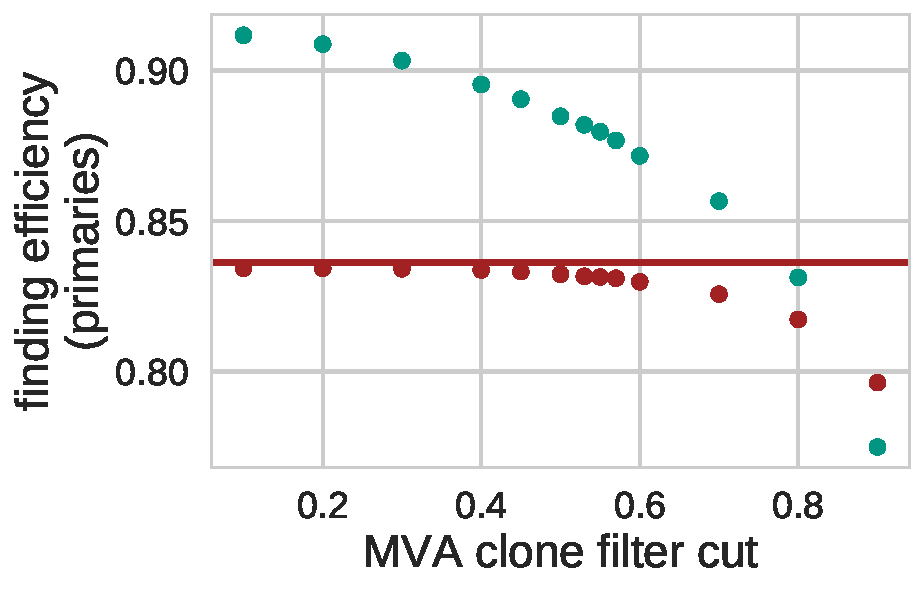
\includegraphics[width=1.0\textwidth]{figures/ca_is_matched_primaries.pdf}\\
      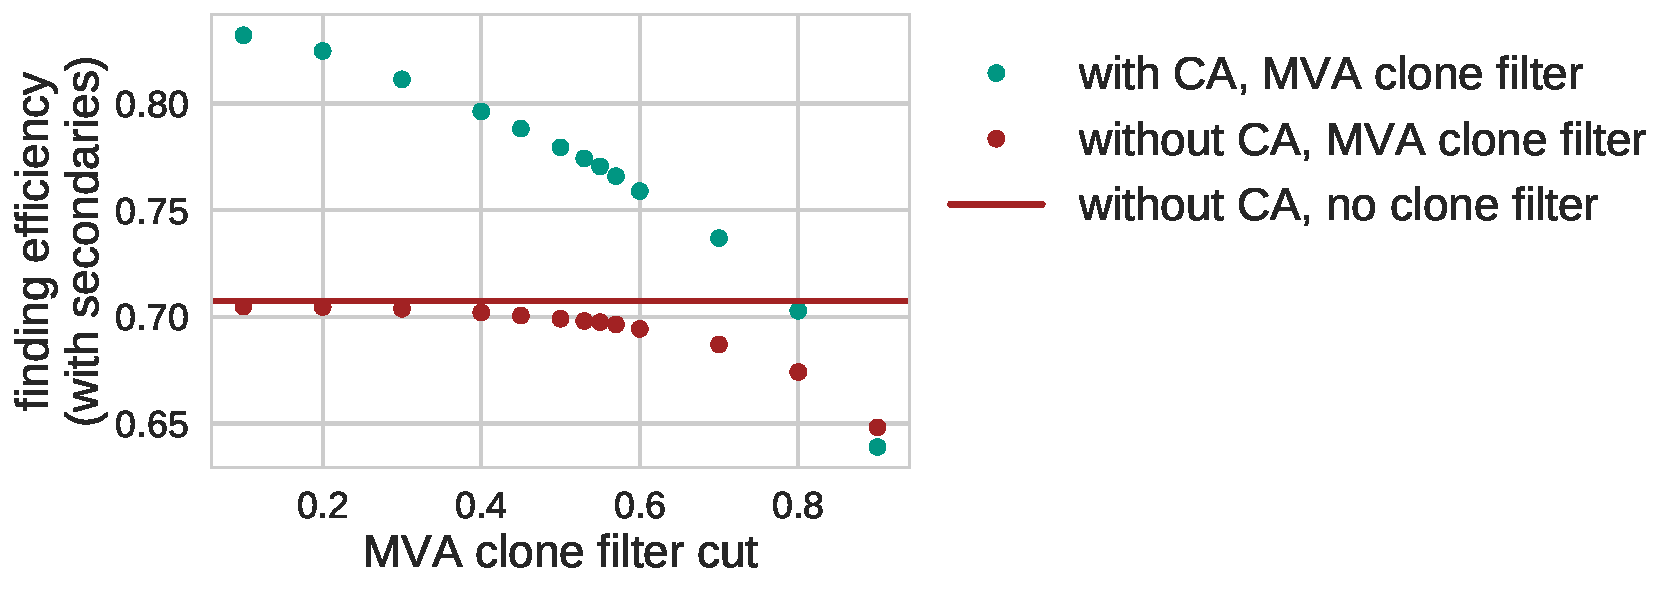
\includegraphics[width=1.0\textwidth]{figures/ca_is_matched_with_secondaries.pdf}
    \end{column}
    \begin{column}{0.3\textwidth}
      \centering
      \includegraphics[width=1.0\textwidth]{figures/ca_clone_rate.pdf}\\
      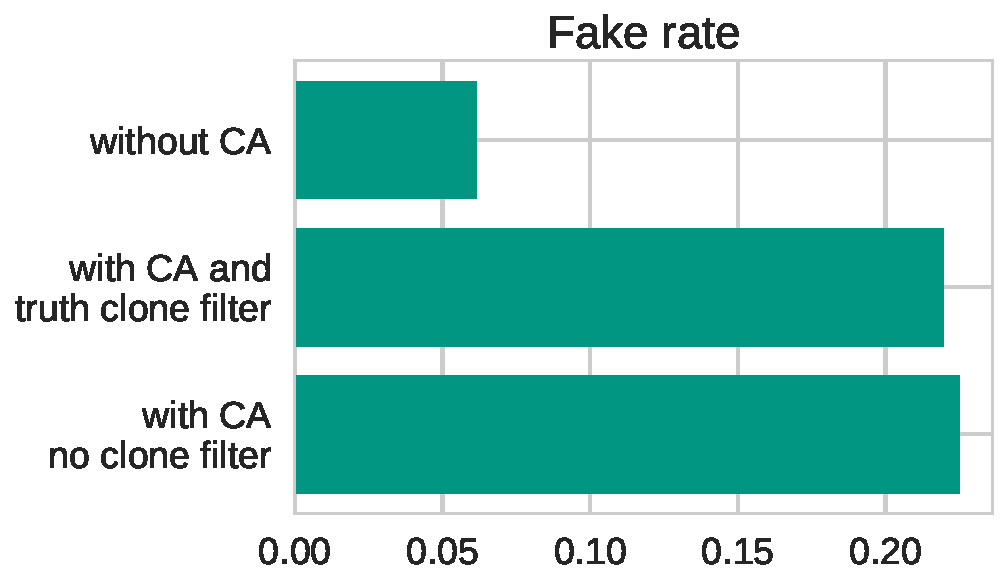
\includegraphics[width=1.0\textwidth]{figures/ca_fake_rate.pdf}
    \end{column}
  \end{columns}
  \begin{columns}
    \begin{column}{.4\textwidth}
      \includegraphics[width=.7\textwidth]{figures/legend_ca_fom_fullreco.pdf}
    \end{column}
    \begin{column}{.6\textwidth}
      good cut around 0.5: with respect to no CA increased finding efficiency and lower fake and
      clone rate
    \end{column}
  \end{columns}  
\end{frame}

\begin{frame}
  \frametitle{Results on full tracking,  including VXD}
  \begin{columns}
    \begin{column}{0.3\textwidth}
      \centering
      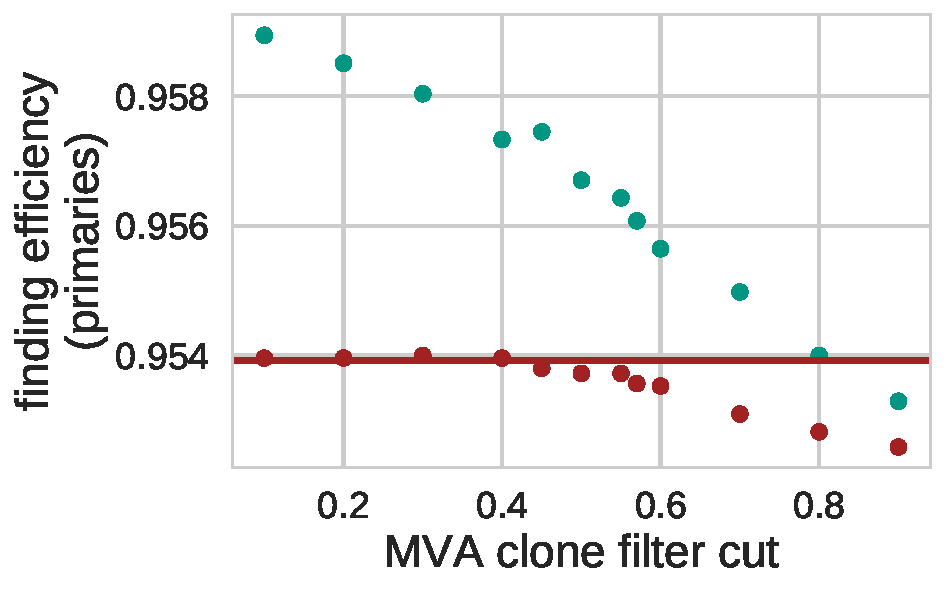
\includegraphics[width=1.0\textwidth]{figures/ca_is_matched_primaries_fullreco.pdf}\\
      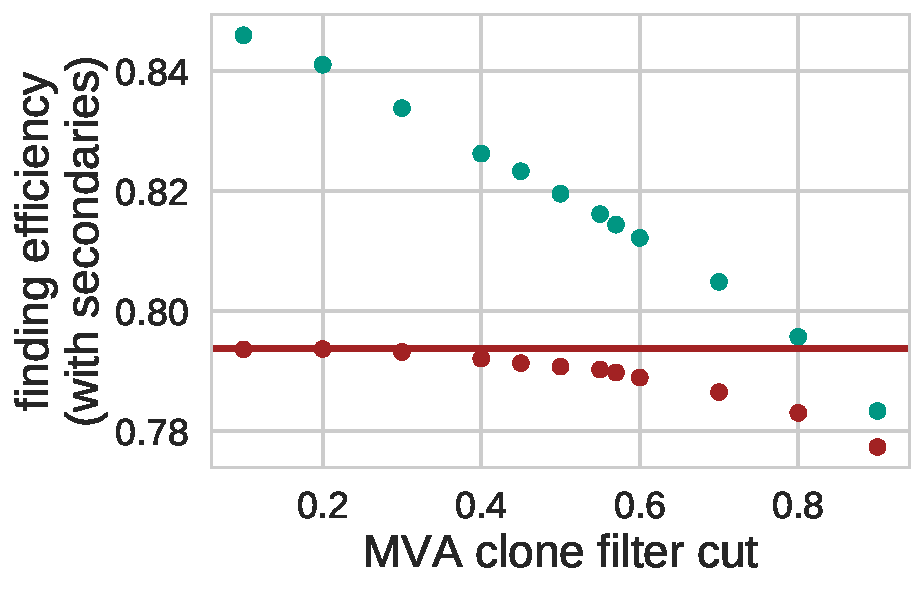
\includegraphics[width=1.0\textwidth]{figures/ca_is_matched_with_secondaries_fullreco.pdf}
    \end{column}
    \begin{column}{0.3\textwidth}
      \centering
      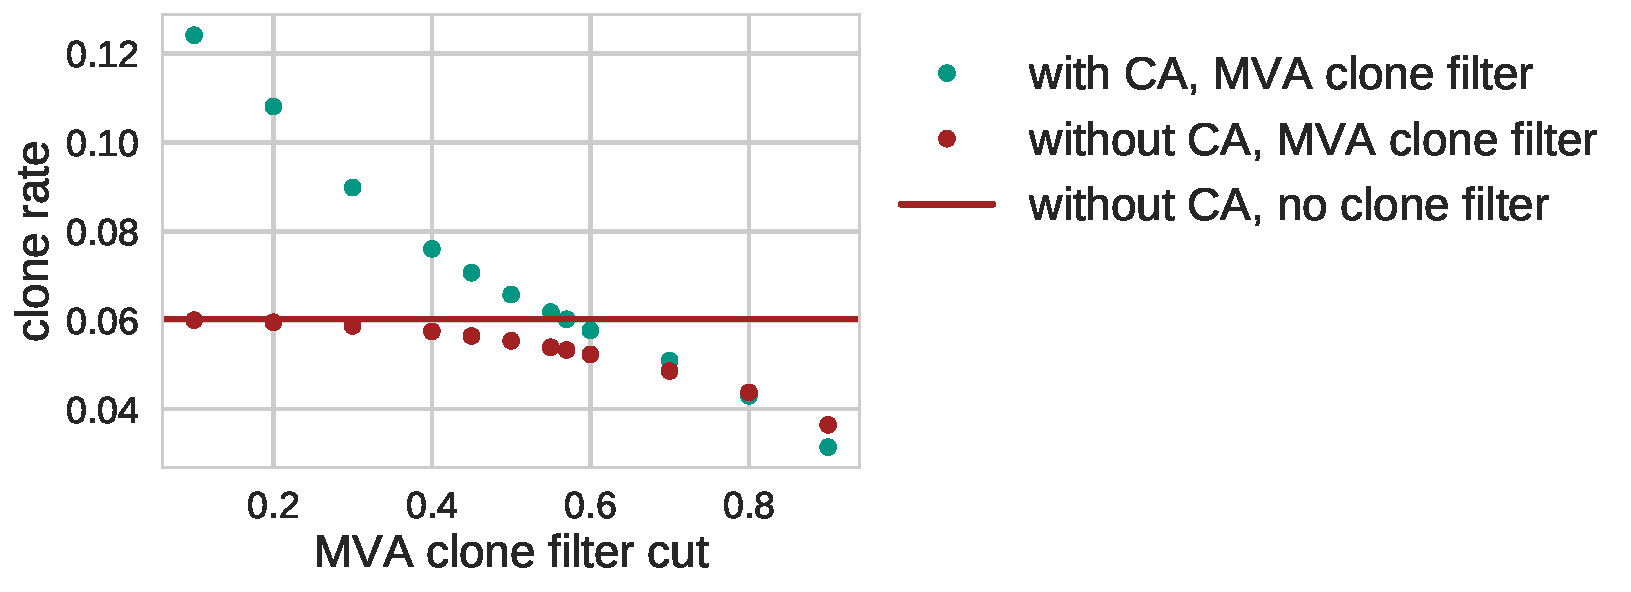
\includegraphics[width=1.0\textwidth]{figures/ca_clone_rate_fullreco.pdf}\\
      \includegraphics[width=1.0\textwidth]{figures/ca_fake_rate_fullreco.pdf}
    \end{column}
  \end{columns}
  \begin{columns}
    \begin{column}{.4\textwidth}
      \includegraphics[width=.7\textwidth]{figures/legend_ca_fom_fullreco.pdf}
    \end{column}
    \begin{column}{.6\textwidth}
       with CA $< \SI{0.5}{\percent}$ improvement on primaries,\\but $> \SI{2}{\percent}$ on secondaries
    \end{column}
  \end{columns}
\end{frame}

\begin{frame}
  \frametitle{Hit efficiency in full tracking}
  \begin{center}
    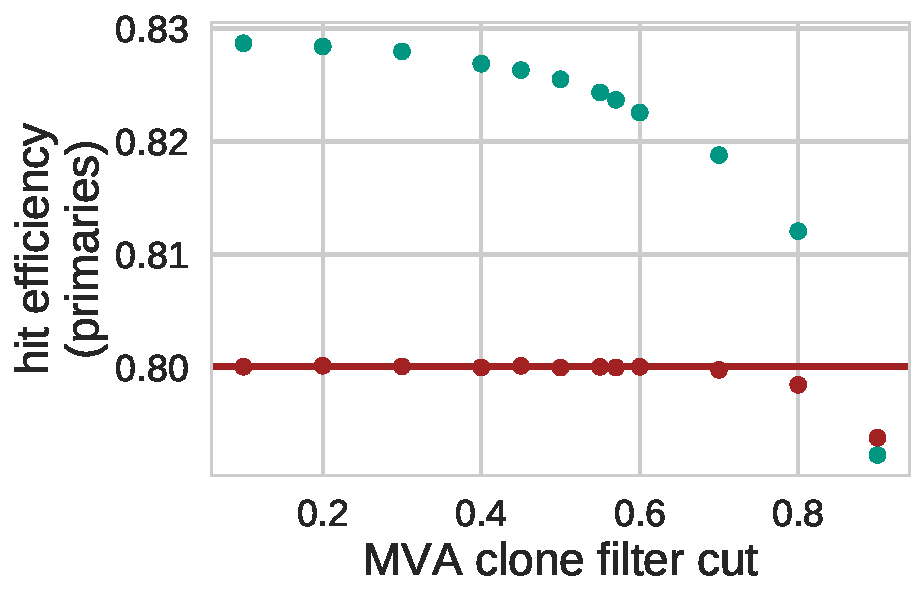
\includegraphics[width=.4\textwidth]{figures/ca_hit_efficiency_primaries_fullreco.pdf}
    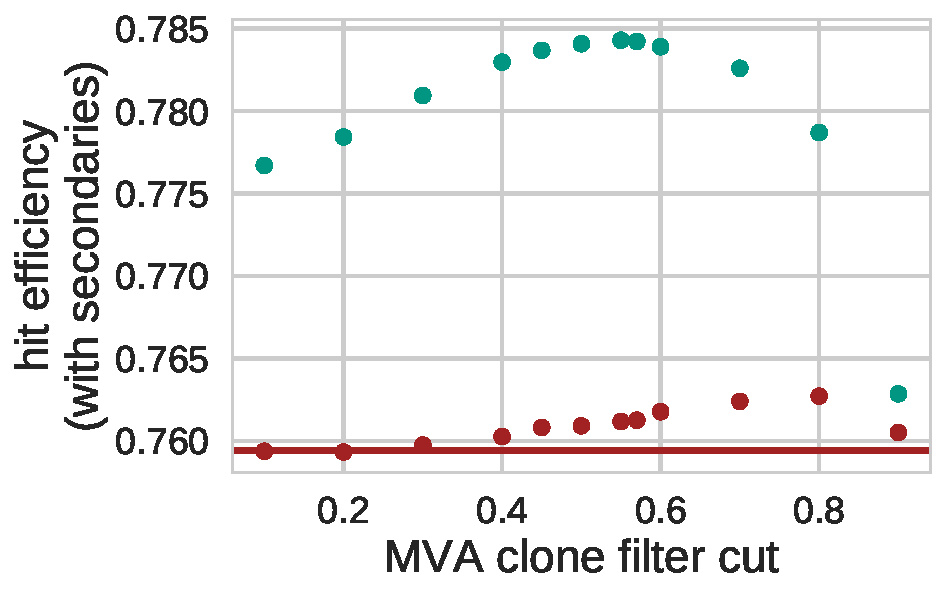
\includegraphics[width=.4\textwidth]{figures/ca_hit_efficiency_with_secondaries_fullreco.pdf}\\
    \includegraphics[width=.3\textwidth]{figures/legend_ca_fom_fullreco.pdf}
  \end{center}
  \begin{itemize}
  \item \SI{2}{\percent}--\SI{3}{\percent} increase in hit efficiency with addition of CA-tracking
  \end{itemize}
\end{frame}

\begin{frame}
  \frametitle{Track distributions}

  \begin{itemize}
  \item In which parameter regions do we \emph{gain} tracks through CA?
  \item Where do we \emph{lose} tracks due to cuts on MVA classifier?
  \item distributions of all tracks (with full tracking):
  \end{itemize}
    
  \begin{columns}
    \begin{column}{.5\textwidth}
      \centering
      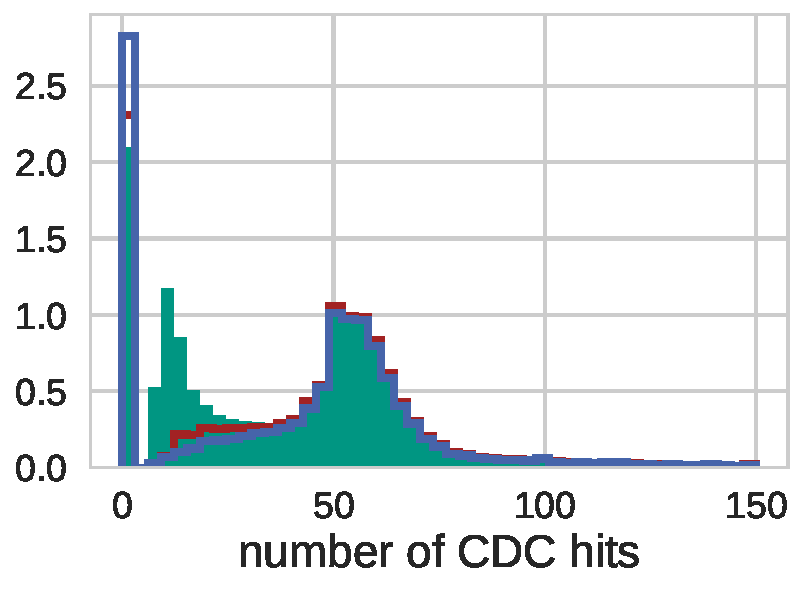
\includegraphics[width=.7\textwidth]{figures/rejected_vs_other_track_distributions_by_found_n_cdc_hits_normed=False_scaleByEvents=True_fullreco.pdf}
      
    \end{column}
    \begin{column}{.5\textwidth}
      \centering
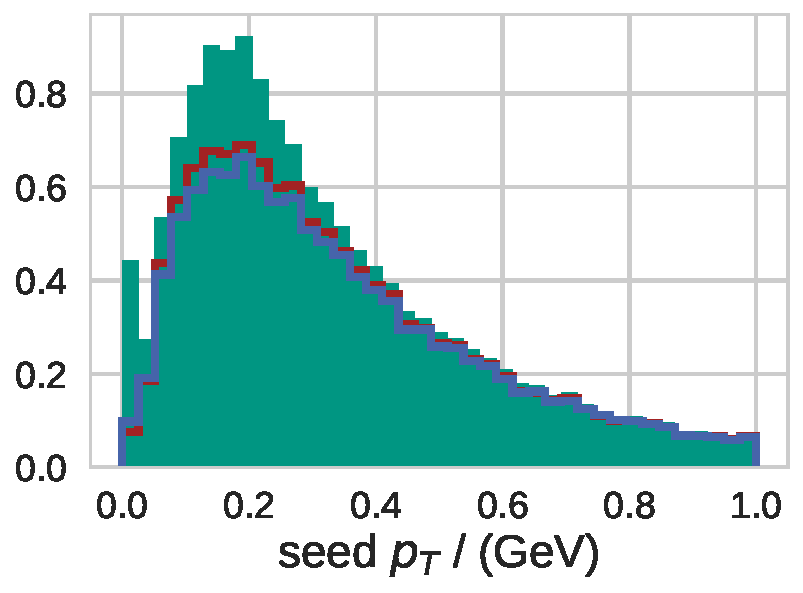
\includegraphics[width=.7\textwidth]{figures/rejected_vs_other_track_distributions_by_found_pt_normed=False_scaleByEvents=True_fullreco.pdf}

    \end{column}
  \end{columns}
  \begin{columns}
    \begin{column}{.5\textwidth}
\includegraphics[width=0.5\textwidth]{figures/legend_rejected_vs_other_track_distributions.pdf}
    \end{column}
    \begin{column}{.5\textwidth}
      $\Rightarrow$\\CA finds low-$p_T$ tracks with low number of hits      
    \end{column}
  \end{columns}
\end{frame}

\begin{frame}
  \frametitle{Finding efficiency profiles with full tracking (including secondaries)}
  \begin{columns}
    \begin{column}{.5\textwidth}
      \centering
      \includegraphics[width=.7\textwidth]{figures/findeff_secondaries_by_pt_truth_fullreco.pdf}\\
      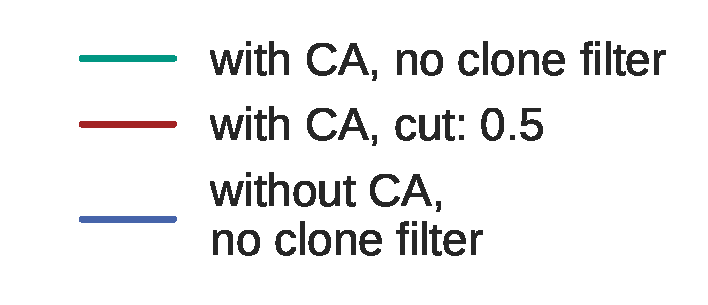
\includegraphics[width=.7\textwidth]{figures/legend_fom_profile.pdf}\\
      $\Rightarrow$ improvements at low $p_T$ and high perigee
    \end{column}    
    \begin{column}{.5\textwidth}
      \centering
      \includegraphics[width=.7\textwidth]{figures/findeff_secondaries_by_d0_truth_fullreco.pdf}\\
      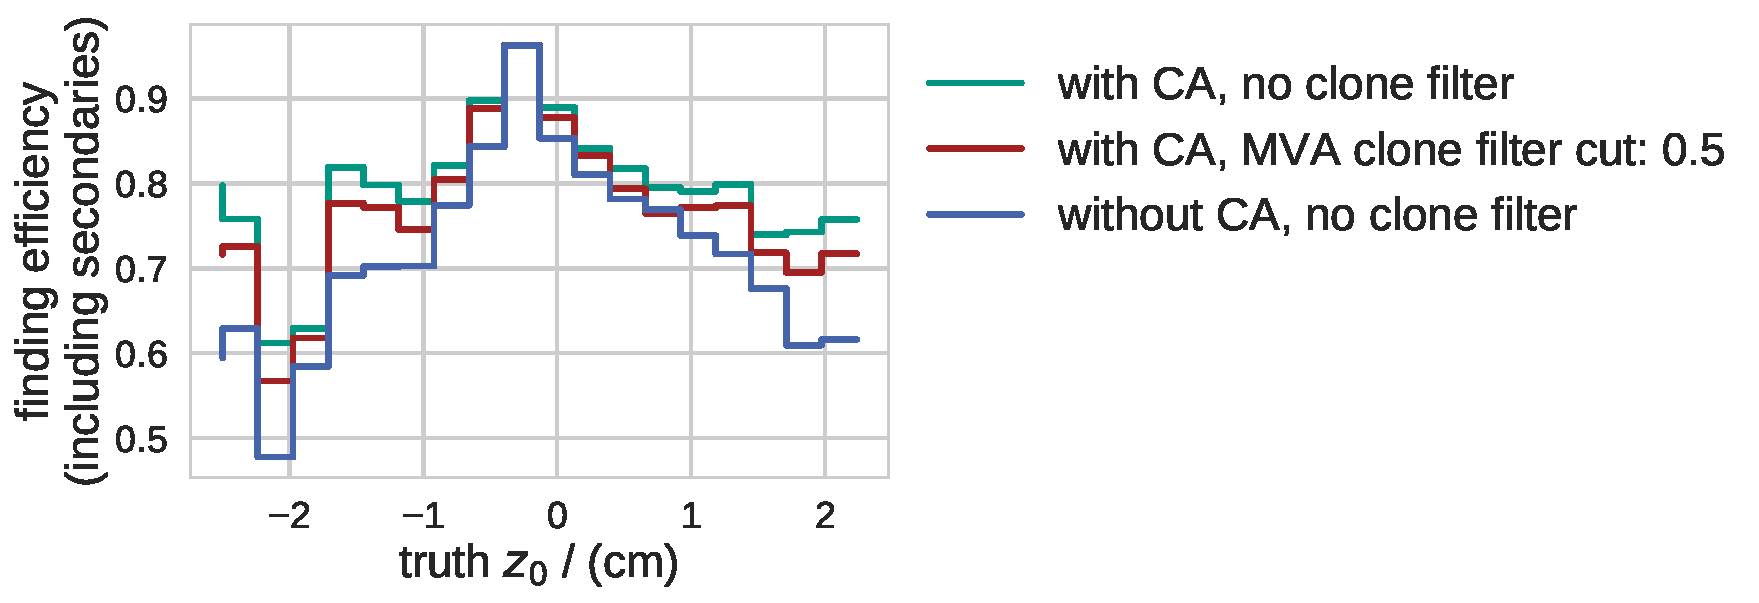
\includegraphics[width=.7\textwidth]{figures/findeff_secondaries_by_z0_truth_fullreco.pdf}
    \end{column}
  \end{columns}
\end{frame}

\begin{frame}
  \frametitle{Hit efficiency profiles with full tracking}
  \begin{columns}
    \begin{column}{.5\textwidth}
      \centering
      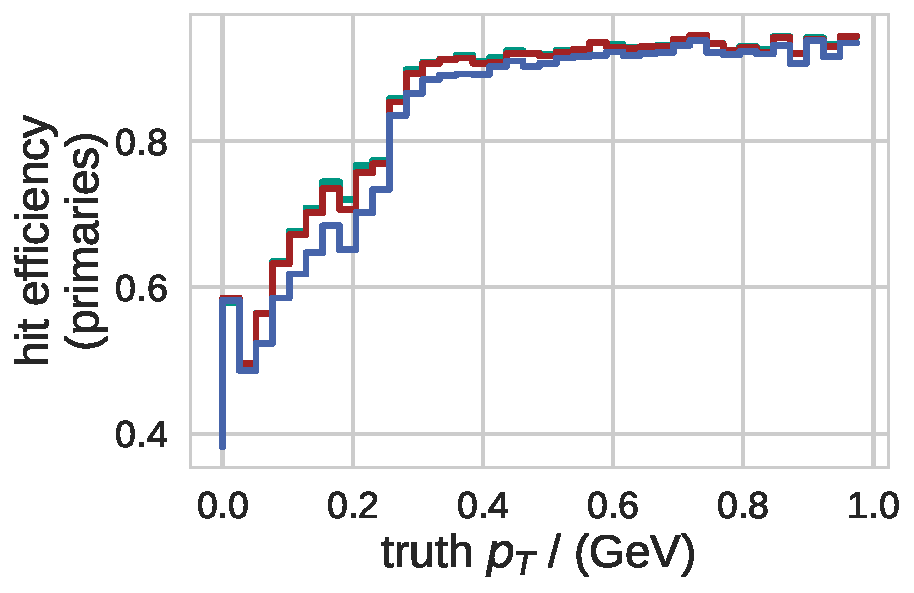
\includegraphics[width=.60\textwidth]{figures/hiteff_by_pt_truth_fullreco.pdf}\\
      \includegraphics[width=.60\textwidth]{figures/hiteff_by_tan_lambda_truth_fullreco.pdf}
    \end{column}    
    \begin{column}{.5\textwidth}
      \centering
      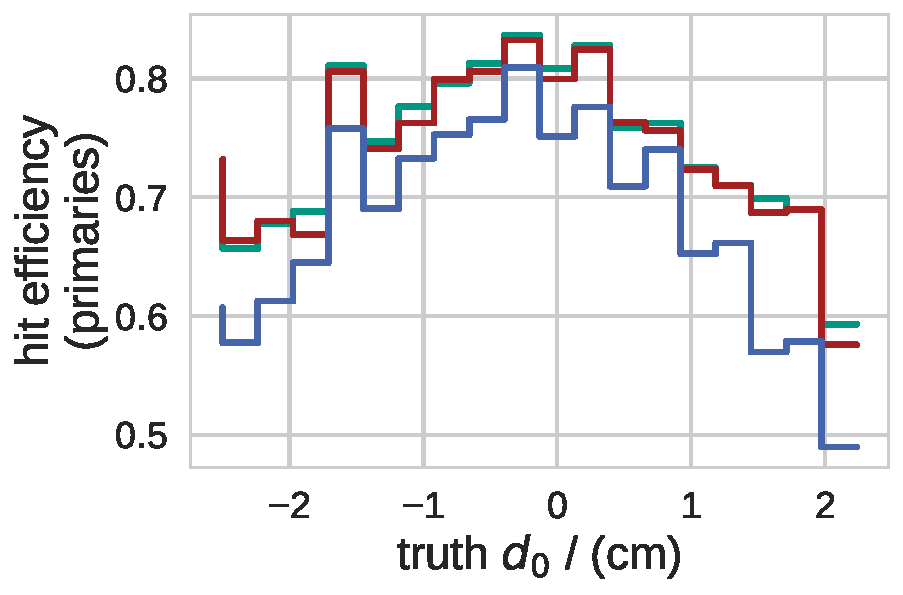
\includegraphics[width=.60\textwidth]{figures/hiteff_by_d0_truth_fullreco.pdf}\\
      \includegraphics[width=.60\textwidth]{figures/hiteff_by_z0_truth_fullreco.pdf}
    \end{column}
  \end{columns}
  \begin{center}
    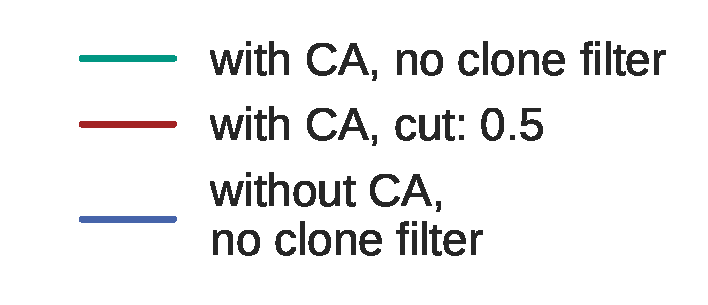
\includegraphics[width=.2\textwidth]{figures/legend_fom_profile.pdf}
  \end{center}
\end{frame}

\begin{frame}
  \frametitle{Summary and outlook}
  \textbf{Summary}
  \begin{itemize}
  \item finding efficiency increases only in CDC-only tracking and full tracking on secondaries
  \item increases hit efficiency, with negligible impact on resolution
  \item problems with clones/fakes solved with on MVA filter
  \item quality indicator stored in \emph{all} CDC reco tracks
  \item current WIP branch: \href{https://stash.desy.de/projects/B2/repos/software/browse?at=refs\%2Fheads\%2Ffeature\%2Fcurler-clone-filtering}{feature/curler-clone-filtering}
  \end{itemize}
  \textbf{Next steps}
  \begin{itemize}
  \item full track QI can be tested with CDC QI of my branch
  \item feature engineering: not difficult, but time sink for after thesis
    \begin{itemize}
    \item use event-wise variables
    \item goal: keep gains from CA
    \end{itemize}
  \item code refactoring for future merge-request, mostly renaming to reflect changed useage
  \end{itemize}
\end{frame}

\appendix
\backupbegin
\begin{frame}
  \centering \huge
  Backup
\end{frame}

\begin{frame}
  \frametitle{Features  used for CDC Track Rejecter training}
  As defined in \texttt{tracking/trackFindingCDC/filters/track/BasicTrackVarSet.h}
  \begin{columns}
    \begin{column}{0.5\textwidth}
      \begin{itemize}
      \item \lstinline{size}
      \item \lstinline{pt}
      \item \lstinline{sz_slope}
      \item \lstinline{drift_length_mean}
      \item \lstinline{drift_length_variance}
      \item \lstinline{drift_length_max}
      \item \lstinline{drift_length_min}
      \item \lstinline{drift_length_sum}
      \item \lstinline{adc_mean}
      \item \lstinline{adc_variance}
      \end{itemize}
    \end{column}
    \begin{column}{0.5\textwidth}
      \begin{itemize}

      \item \lstinline{adc_max}
      \item \lstinline{adc_min}
      \item \lstinline{adc_sum}
      \item \lstinline{empty_s_mean}
      \item \lstinline{empty_s_variance}
      \item \lstinline{empty_s_max}
      \item \lstinline{empty_s_min}
      \item \lstinline{empty_s_sum}
      % \item \lstinline{has_matching_segment}
      \item \lstinline{s_range}
      \end{itemize}      
    \end{column}
  \end{columns}
\end{frame}

\begin{frame}
  \frametitle{Finding efficiency profiles with full tracking on primaries}
  \begin{columns}
    \begin{column}{.5\textwidth}
      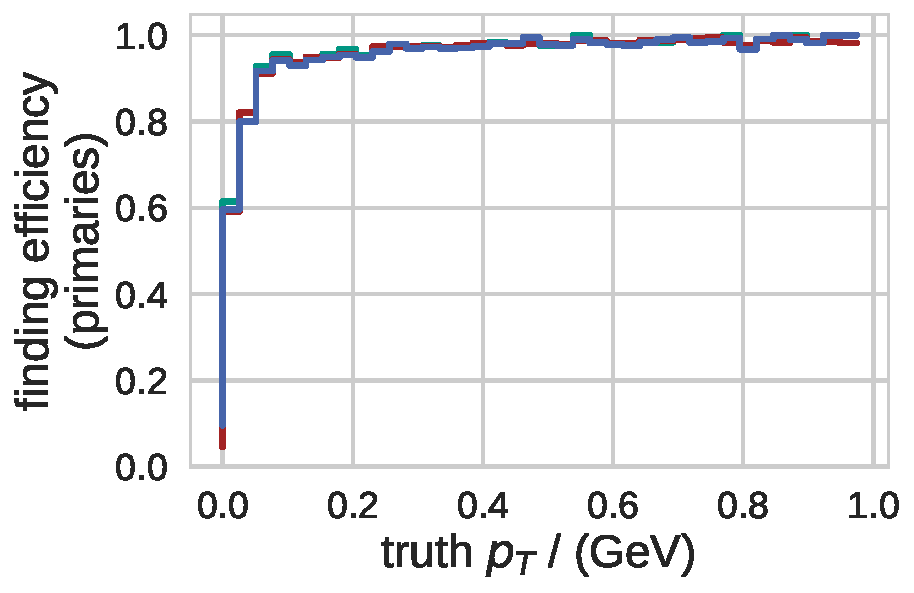
\includegraphics[width=.7\textwidth]{figures/findeff_by_pt_truth_fullreco_trainedWithFakes.pdf}\\
      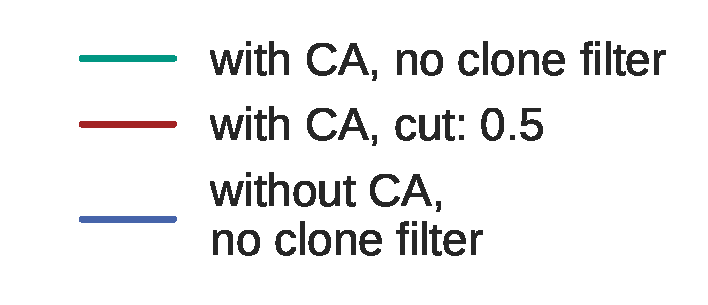
\includegraphics[width=.7\textwidth]{figures/legend_fom_profile.pdf}\\
      % $\Rightarrow$ improvements at low $p_T$ and high perigee
    \end{column}    
    \begin{column}{.5\textwidth}
      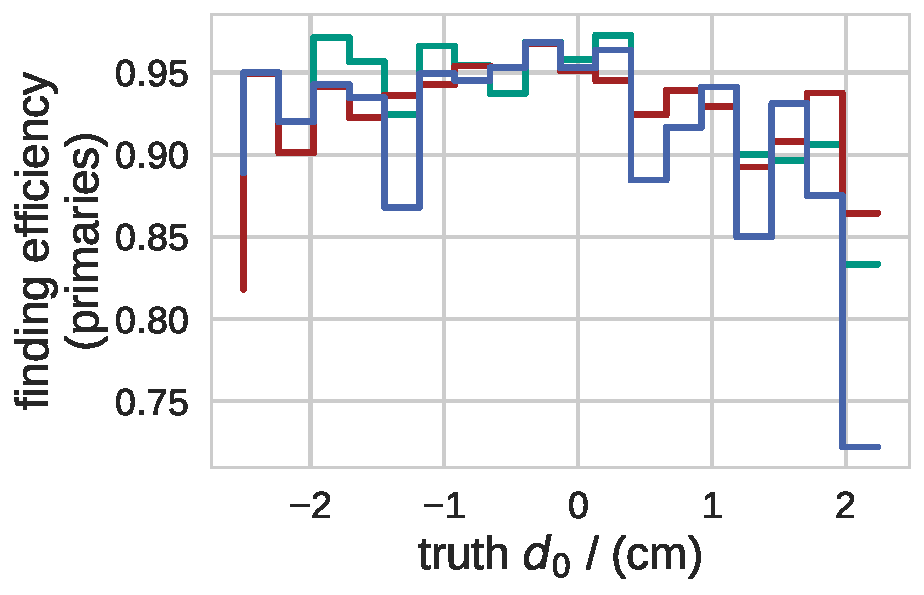
\includegraphics[width=.7\textwidth]{figures/findeff_by_d0_truth_fullreco_trainedWithFakes.pdf}\\
      \includegraphics[width=.7\textwidth]{figures/findeff_by_z0_truth_fullreco_trainedWithFakes.pdf}
    \end{column}
  \end{columns}
\end{frame}

\begin{frame}
  \frametitle{Clone rate profiles in full tracking}
  \begin{columns}
    \begin{column}{.5\textwidth}
      \centering    
      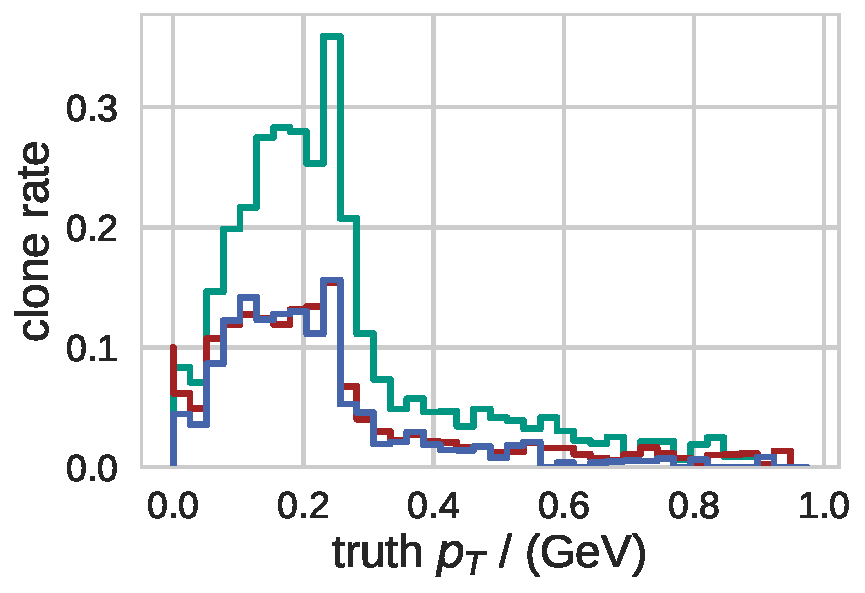
\includegraphics[width=.55\textwidth]{figures/clone_rate_by_pt_truth_fullreco_trainedWithFakes.pdf}\\
      \includegraphics[width=.55\textwidth]{figures/clone_rate_by_tan_lambda_truth_fullreco_trainedWithFakes.pdf}
    \end{column}

    \begin{column}{.5\textwidth}
      \centering
      \includegraphics[width=.55\textwidth]{figures/clone_rate_by_z0_truth_fullreco_trainedWithFakes.pdf}\\
      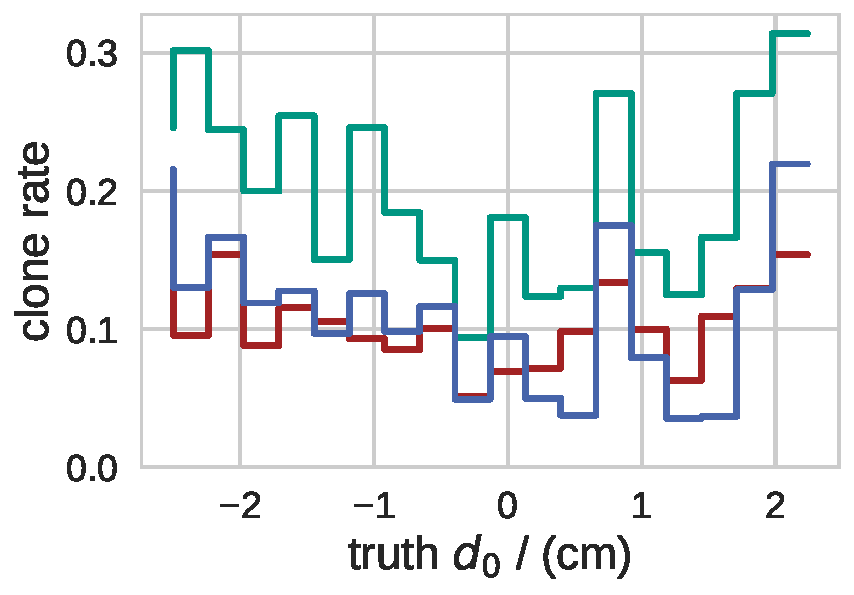
\includegraphics[width=.55\textwidth]{figures/clone_rate_by_d0_truth_fullreco_trainedWithFakes.pdf}
    \end{column}
  \end{columns}
  \begin{center}
    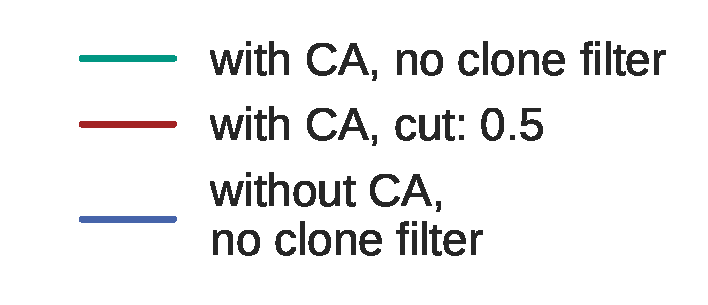
\includegraphics[width=.25\textwidth]{figures/legend_fom_profile.pdf}\\
  \end{center}
\end{frame}

\begin{frame}
  \frametitle{Fake rate profiles in full tracking}
  \begin{columns}
      \begin{column}{.5\textwidth}
      \centering
      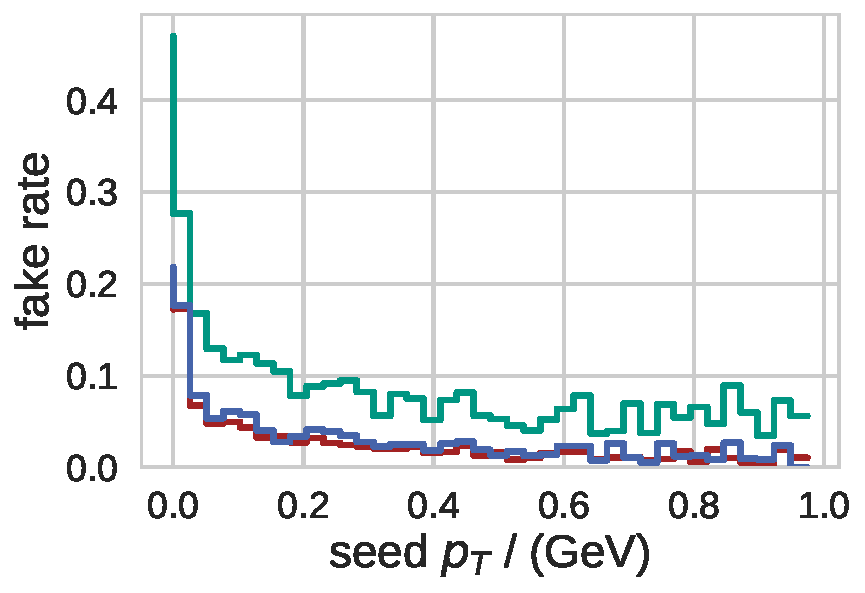
\includegraphics[width=.55\textwidth]{figures/fake_rate_by_pt_truth_fullreco_trainedWithFakes.pdf}\\
      \includegraphics[width=.55\textwidth]{figures/fake_rate_by_tan_lambda_truth_fullreco_trainedWithFakes.pdf}
    \end{column}

    \begin{column}{.5\textwidth}
      \centering
      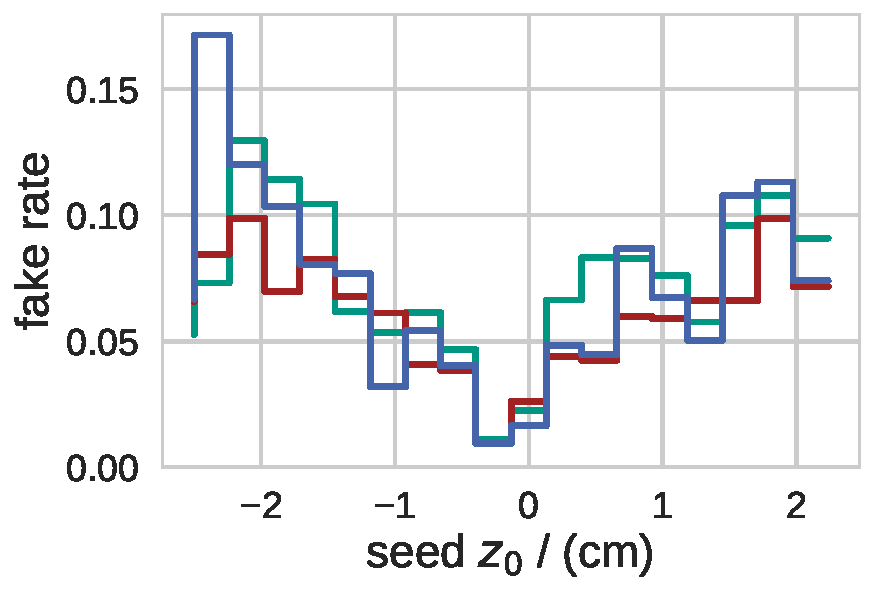
\includegraphics[width=.55\textwidth]{figures/fake_rate_by_z0_truth_fullreco_trainedWithFakes.pdf}\\
      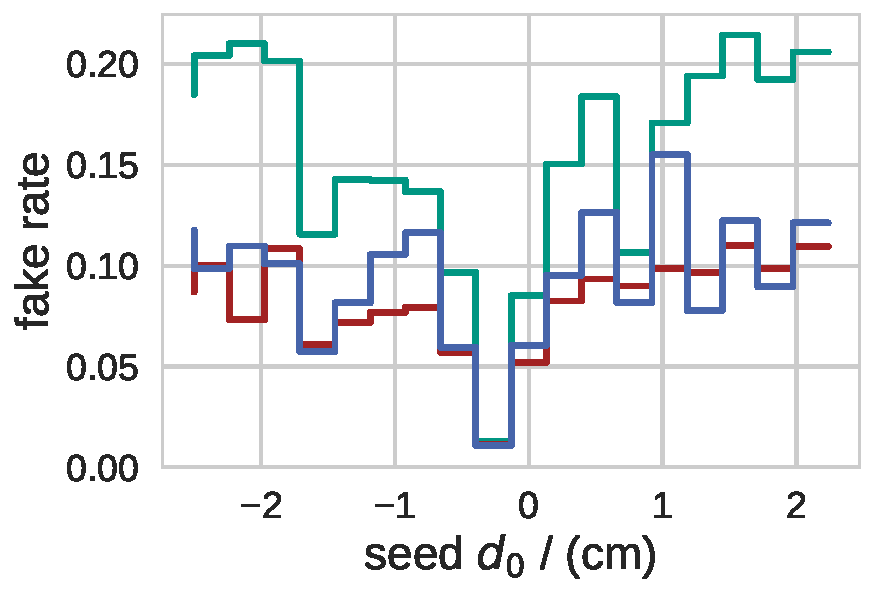
\includegraphics[width=.55\textwidth]{figures/fake_rate_by_d0_truth_fullreco_trainedWithFakes.pdf}      
    \end{column}
  \end{columns}
  \begin{center}
    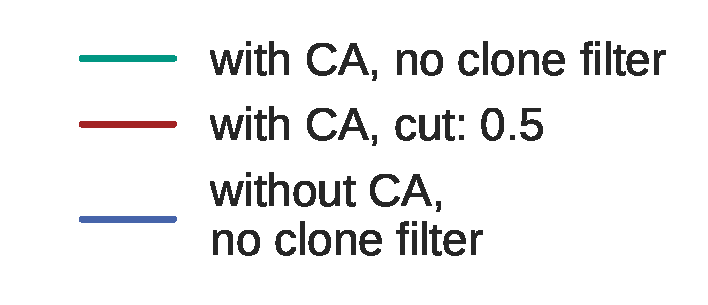
\includegraphics[width=.25\textwidth]{figures/legend_fom_profile.pdf}\\
  \end{center}  
\end{frame}

\begin{frame}
  \frametitle{Hit efficiency profiles on matched hits only}
  \begin{columns}
    \begin{column}{.5\textwidth}
      \centering
      \includegraphics[width=.65\textwidth]{figures/hiteff_on_matched_by_pt_truth_fullreco_trainedWithFakes.pdf}\\
      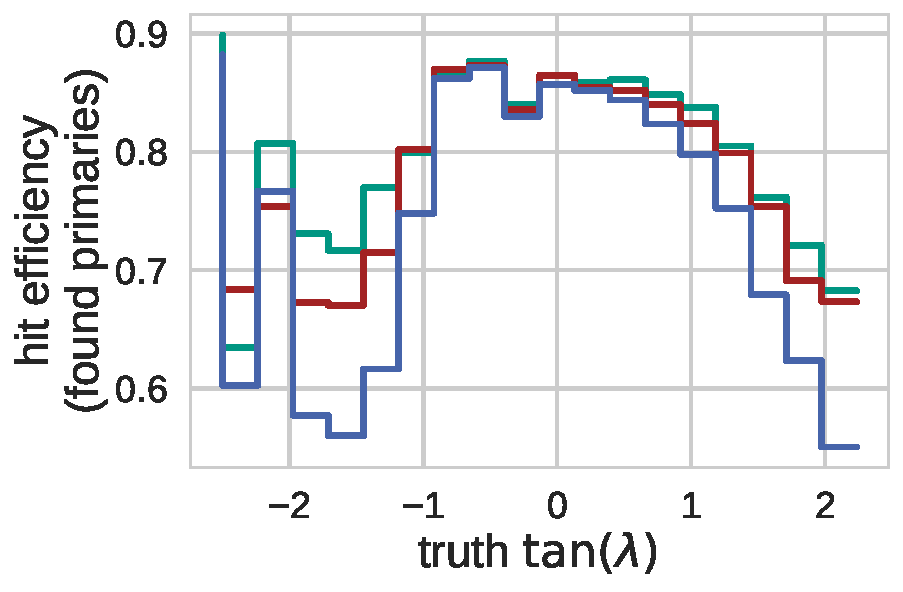
\includegraphics[width=.65\textwidth]{figures/hiteff_on_matched_by_tan_lambda_truth_fullreco_trainedWithFakes.pdf}
    \end{column}    
    \begin{column}{.5\textwidth}
      \centering
      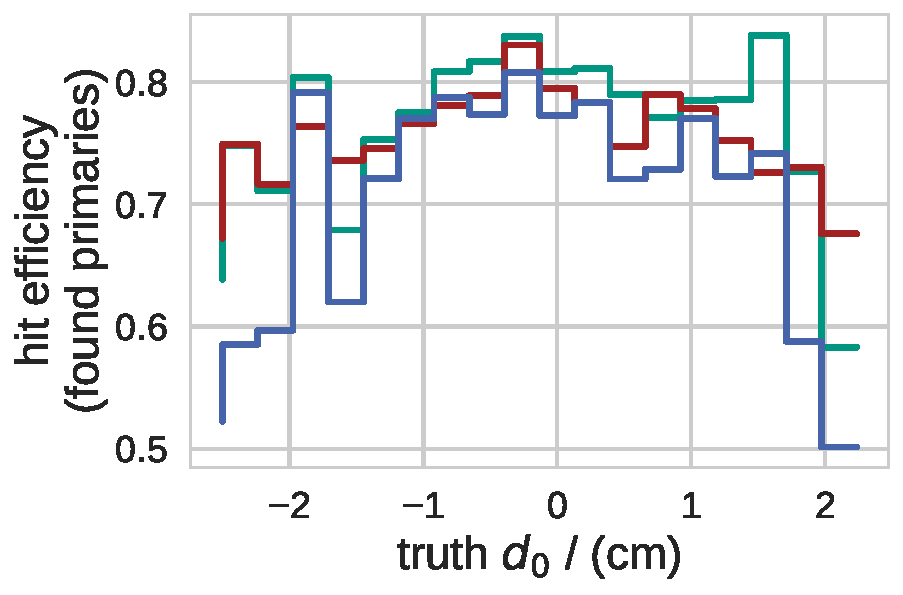
\includegraphics[width=.65\textwidth]{figures/hiteff_on_matched_by_d0_truth_fullreco_trainedWithFakes.pdf}\\
      \includegraphics[width=.65\textwidth]{figures/hiteff_on_matched_by_z0_truth_fullreco_trainedWithFakes.pdf}
    \end{column}
  \end{columns}
  \begin{center}
    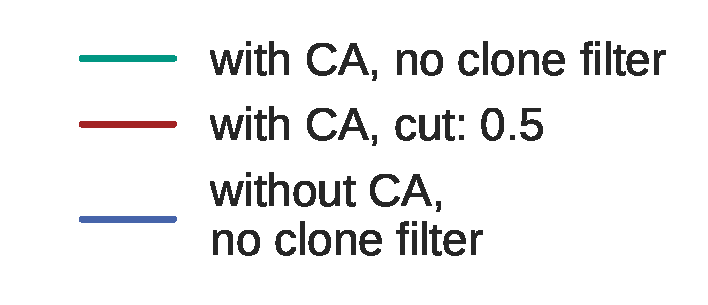
\includegraphics[width=.2\textwidth]{figures/legend_fom_profile.pdf}
  \end{center}

\end{frame}

\begin{frame}[allowframebreaks]
  \frametitle{Plots from recording filter outputt}
  \includegraphics[width=0.4\textwidth]{figures/clone_multiplicities.pdf}\\
  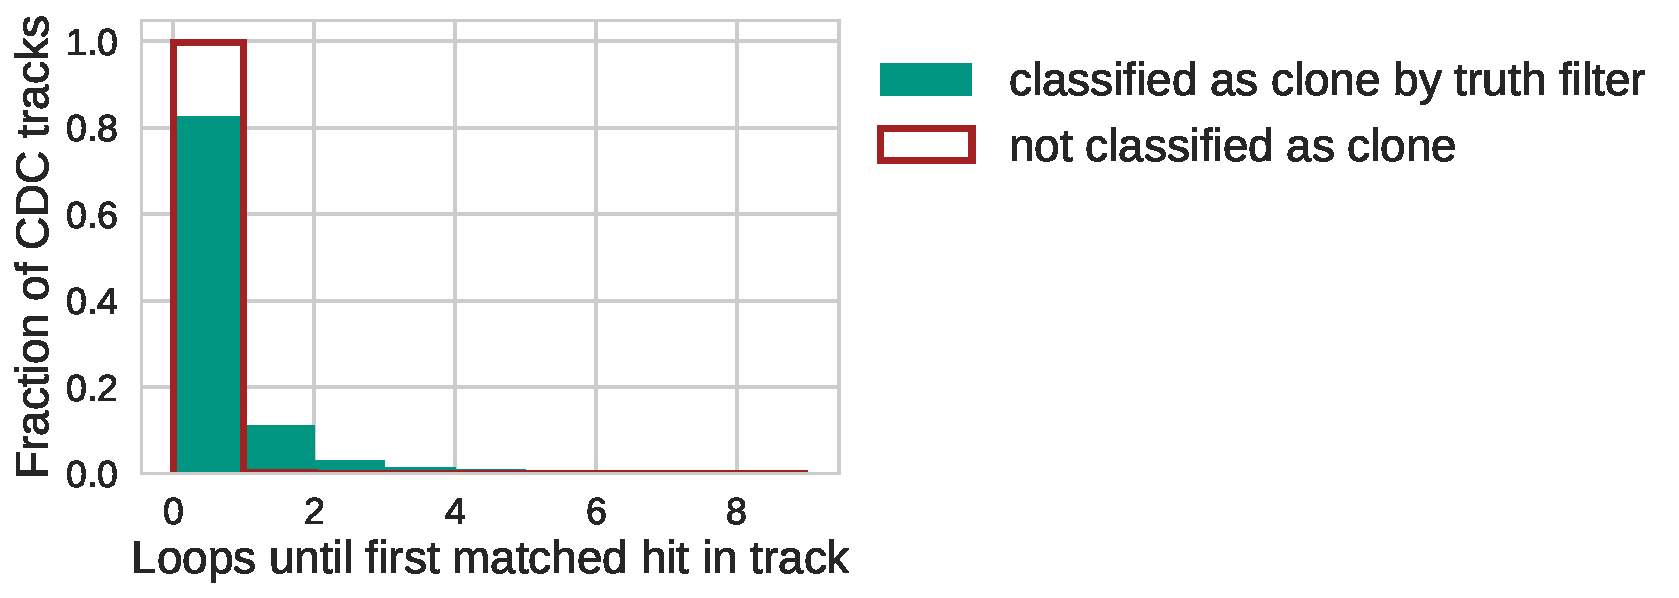
\includegraphics[width=0.7\textwidth]{figures/loop_numbers.pdf}\\
  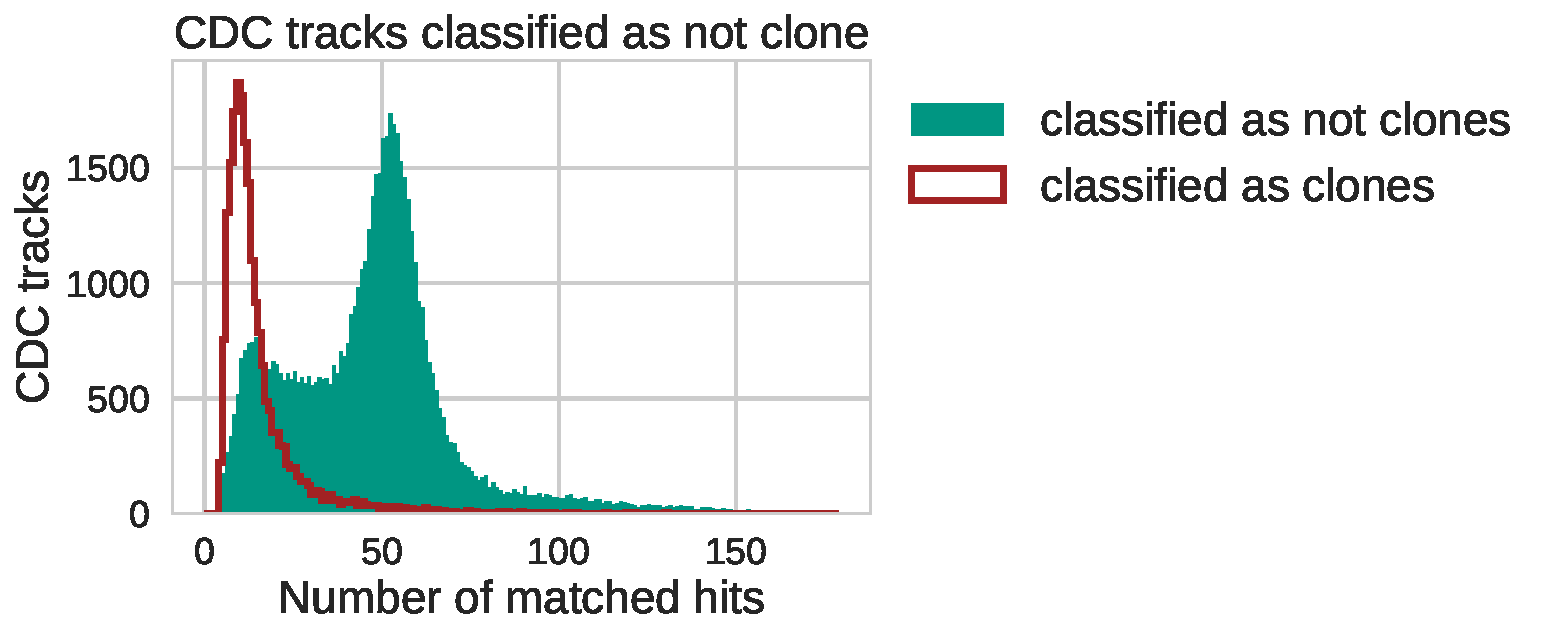
\includegraphics[width=0.7\textwidth]{figures/matched_hits.pdf}\\
\end{frame}

\end{document}

%%% Local Variables:
%%% coding: utf-8
%%% mode: LaTeX
%%% TeX-engine: default
%%% TeX-master: t
%%% ispell-dictionary: "english"
%%% synosaurus-backend: synosaurus-backend-wordnet
%%% fill-column: 100
%%% End:
%%% Local Variables: